

The following instructions may vary according to the vendor, version, and specifications of the operating system being used. Please adapt them as necessary. Consult the operating system documentation for details.

\begin{enumerate}
\item From the command shell, navigate to the directory where you saved the setup file you downloaded. 
\item Launch the installation program by starting the script:\\
\bxshell{./setup.sh}
  
Because the files are being decompressed, this make take some time.  
  \item The license agreement will appear. Read it and accept it to continue.  
You can view and print this license later. It is saved in the \jb{} installation directory and is called license-agreement.txt.   
\item At the next dialog, choose where to install \jb{}. You can search or enter a directory or use the default. Click \bxcaption{Next}.

\item Choose the components to be installed.
You can install the \gdserver{} (the server component) and the client on different machines if you want to. If this is the case, carry out the installation for the other component (server or \gdserver{}) later. 

To be able to access the manual as a .pdf file and to  print it  out, install the  \jb{} documentation. Click \bxcaption{Next}.


\item Choose the directory in which symlinks for \jb{}{} should be created (\bxfigref{figSymlinks}). The directory must be writable by the user installing the program, i.e. a non-adminstrator may use his home directory. Symlinks should be created in a folder contained in  the \$PATH variable.

If you do not want to create symlinks, check the box for this option. Click \bxcaption{Next} to continue.  

  \begin{center}
  \begin{figure}[h]
    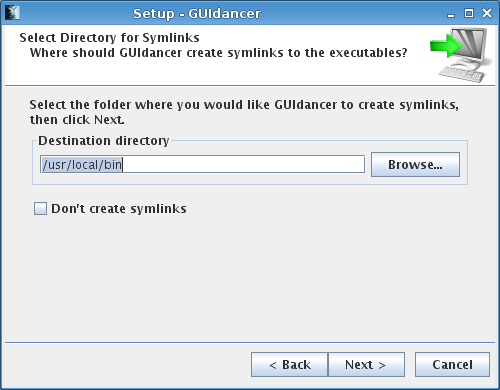
\includegraphics[width=10cm]{Windows/PS/symlinks}
    \caption{Configuring symlinks location}
    \label{figSymlinks}
  \end{figure}
  \end{center}

\item The selected components will  be installed.
\item Once the installation is finished, a dialog appears to confirm this. 

From this dialog you can also opt to start the configuration tool 
%\gddb initialization
 and license administrator after finishing the installation
process. 

We recommend starting the license administrator automatically, especially if you are a first-time user. If you want to  customize your installation, it is a good
idea to run the configuration tool before using 
%the CreateDB tool or 
the license administrator. See later \bxpref{custInst} for details on the configuration tool.
 

\bxtipp{Configuration details can also be changed at a later point using the configuration tool (\bxshell{gdconfig}). }

\item Click \bxcaption{Finish} to exit the installation wizard. 
\item You can  now use the configuration tool (optional),
% and you must create a database using the createDB tool, 
and you must then start the license administrator to request and add licenses.  

\end{enumerate}
